\documentclass{lucas-report}

\title{CSED490F Lab: Autograd}
\author{Team 4: Yunkyu Lee (20210733), Hyeonu Cho (20230740)}
\date{September 16, 2025}

\NewDocumentCommand{\jacobian}{}{\ensuremath{\text{J}}}

\addbibresource{lab2_autograd_team4.bib}

\begin{document}
\maketitle

\section{Automatic Differentiation}\label{sec:autodiff}

Reverse-mode automatic differentiation performs
back-to-front accumulation of local gradients based on the chain rule.
% Consider a function $f : \mathbb{R}^{n} \mapsto \mathbb{R}^m$,
% and its $m \times n$ Jacobian $\jacobian_f$.
% For some $y = f(x)$, suppose we know $\pdv{\Ell}/{y}$,
% the gradient of some scalar value $\Ell$ w.r.t. $y$.
% Then, we can obtain $\pdv{\Ell}/{x}$ as a vector-Jacobian product (VJP):
% \[
%   \pdv{\Ell}{x} = \left(\pdv{\Ell}{y}\right)^\top \jacobian_f (x)
% \]
% As $\jacobian_{f_1 \circ f_2} = \jacobian_{f_1} \circ J_{f_2}$,
% we can chain the above VJP in order to obtain gradients of composed functions.
% Therefore, knowing the local gradients of function outputs w.r.t. their inputs
% is sufficient for reverse-mode automatic differentiation.

% \subsection{Basic Operations}

We omit the definitions and the local gradients of the
\texttt{Add}, \texttt{Mul}, \texttt{Pow}, \texttt{Log}, and \texttt{Sum} operations as they are trivial,
and show \texttt{ReLU} as an example.
% \begin{equation}
%   \texttt{Add}(x, y) = x + y,
%   \quad \pdv{\texttt{Add}}{x} = 1,
%   \quad \pdv{\texttt{Add}}{y} = 1
% \end{equation}
% \begin{equation}
%   \texttt{Mul}(x, y) = x \times y,
%   \quad \pdv{\texttt{Mul}}{x} = y,
%   \quad \pdv{\texttt{Mul}}{y} = x
% \end{equation}
% \begin{equation}
%   \texttt{Pow}(x, y) = x^y,
%   \quad \pdv{\texttt{Pow}}{x} = yx^{y-1},
%   \quad \pdv{\texttt{Pow}}{y} = x^y \log x
% \end{equation}
% \begin{equation}
%   \texttt{Log}(x) = \log x,
%   \quad \pdv{\texttt{Log}}{x} = x^{-1}
% \end{equation}
\[
  \texttt{ReLU}(x) = \max(x, 0),
  \quad \pdv{\texttt{ReLU}(x)}{x} =
  \begin{cases}
    1 & x > 0, \\
    0 & x < 0
  \end{cases}
\]
% \begin{equation}
%   \texttt{Sum}(x) = \sum_{i} x_i
%   % TODO - any other way to represent this better? matrix whose every elem is 1?
%   \quad \pdv{\texttt{Sum}}{x} = 1
% \end{equation}

\subsection{Matrix Multiplication}

We define \(\texttt{MatMul}\) as the matrix multiplication operator.
Let $z = \texttt{MatMul}(x, y)$ for \(x \in \mathbb{R}^{N \times D}\) and \(y \in \mathbb{R}^{D \times M}\).
Then, each element of \(z \in \mathbb{R}^{N \times M}\) is computed as \(z_{n,m} = \sum_d x_{n,d}\,y_{d,m}\).
Any element \(x_{n,m}\) of \(x\) only contributes to row $n$ of \(z\):
\[
  z_{n,*} =
  \begin{bmatrix}
    \sum_d x_{n,d}\,y_{d,1} & \sum_d x_{n,d}\,y_{d,2} & \cdots & \sum_d x_{n,d}\,y_{d,M-1} & \sum_d x_{n,d}\,y_{d,M}
  \end{bmatrix}
\]
This gives \(\pdv{\Ell}/{x}\) as the following:
\[
  \pdv{\Ell}{x_{n,d}} =
  \sum_m \pdv{\Ell}{{z_{n,m}}} \pdv{z_{n,m}}{x_{n,d}} =
  \sum_m \pdv{\Ell}{{z_{n,m}}} y_{d,m} =
  \pdv{\Ell}{{z_{n,*}}} y_{d,*}^\top
\]
Finally, we obtain the backpropagation rules for \texttt{MatMul}.
\[
  \pdv{\Ell}{x} = \pdv{\Ell}{{\texttt{MatMul}(x, y)}} y^\top, \quad
  \pdv{\Ell}{y} = x^\top \pdv{\Ell}{{\texttt{MatMul}(x, y)}}
\]

\subsection{Classification}

\textbf{Softmax.} Following \cite{accurate-softmax}, we implement the softmax function with a shift for numerical stability.
This shift has no impact on the output result or the gradient.
\[
  \texttt{Softmax}(x)_j = \frac{\exp{(x_j - s)}}{\sum_i{\exp{(x_i - s)}}}
\]
By simple differentiation, we can obtain \(\pdv{\texttt{Softmax}(x)_i}/{x_j}\) for $i=j$ and $i\neq j$ as the following:
\[
  \pdv{\texttt{Softmax}(x)_j}{x_j} = \texttt{Softmax}(x)_j - \texttt{Softmax}(x)_j^2,
  \quad \pdv{\texttt{Softmax}(x)_i}{x_j} = - \texttt{Softmax}(x)_i \texttt{Softmax}(x)_j
\]

% We derive the local gradient \(\pdv{\texttt{Softmax}(x)_j}/{x_j}\) with the following steps:
% \[
%   \begin{aligned}
%     \pdv{\texttt{Softmax}(x)_j}{x_j} & = \frac{\exp x_j \sum_i{\exp{x_i}} - \exp x_j \pdv*{\sum_i{\exp{x_i}}}{x_j}}{\bigl(\sum_i{\exp{x_i}}\bigr)^2} \\
%     & = \frac{\exp x_j \sum_i{\exp{x_i}} - (\exp x_j)^2}{\bigl(\sum_i{\exp{x_i}}\bigr)^2}                           \\
%     & = \texttt{Softmax}(x)_j - \texttt{Softmax}(x)_j^2
%   \end{aligned}
% \]
% Similarly, we can obtain \(\pdv{\texttt{Softmax}(x)_i}/{x_j} = - \texttt{Softmax}(x)_i \texttt{Softmax}(x)_j\).
% \[
%   \pdv{\texttt{Softmax}(x)_i}{x_j} = - \texttt{Softmax}(x)_i \texttt{Softmax}(x)_j
% \]

Using the above gradients, we can derive a backpropagation rule in matrix form:
\[
  \begin{aligned}
    \pdv{\Ell}{x_j} & = \sum_i \pdv{\Ell}{\texttt{Softmax}(x)_i} \pdv{\texttt{Softmax}(x)_i}{x_j} \\
    & = \pdv{\Ell}{\texttt{Softmax}(x)_j} \bigl( \texttt{Softmax}(x)_j - \texttt{Softmax}(x)_j^2 \bigr)
    - \sum_{i \neq j } \pdv{\Ell}{\texttt{Softmax}(x)_i} \texttt{Softmax}(x)_i \texttt{Softmax}(x)_j \\
    & = \texttt{Softmax}(x)_j \left( \pdv{\Ell}{\texttt{Softmax}(x)_j} - \sum_i \pdv{\Ell}{\texttt{Softmax}(x)_i}\texttt{Softmax}(x)_i \right)
  \end{aligned}
\]

\textbf{Negative log-likelihood.} The negative log-likelihood loss (with log-probability input) is defined as the following,
with trivial local gradients:
\[
  \texttt{NLLLoss}(\log\hat{p}, p) = -\sum_i p_i \log \hat{p}_i, \quad
  \pdv{{\texttt{NLLLoss}(\log\hat{p}, p)}}{p} = -\log\hat{p}, \quad
  \pdv{{\texttt{NLLLoss}(\log\hat{p}, p)}}{\log\hat{p}} = -p
\]

\textbf{Cross-entropy.} The cross-entropy loss (with logit inputs) can be seen as a composition of \texttt{Softmax} and \texttt{NLLLoss}.
\[
  \texttt{CrossEntropyLoss}(\hat{x}, p) = \texttt{NLLLoss}\Bigl(\log\bigl(\texttt{Softmax}(\hat{x})\bigr), p\Bigr) = -\sum_i p_i \log \bigl(\texttt{Softmax}(\hat{x_i})\bigr)
\]
The local gradients can be found accordingly by the chain rule on \texttt{Log}, \texttt{Softmax}, and \texttt{NLLLoss}.
\[
  \begin{aligned}
    \pdv{\texttt{CrossEntropyLoss}(\hat{x}, p)}{\hat{x}_j} = \texttt{Softmax}(\hat{x})_j - p_j,
    \quad \pdv{\texttt{CrossEntropyLoss}(\hat{x}, p)}{p_j} = - \log \bigl( \texttt{Softmax}(\hat{x}) \bigr)_j
  \end{aligned}
\]

\section{MNIST Classification}

Utilizing the operators described in \autoref{sec:autodiff},
we train an MLP $f_\theta$ to perform classification on the MNIST dataset.
The MLP architecture used is shown below.
\begin{figure}[h]
  \centering
  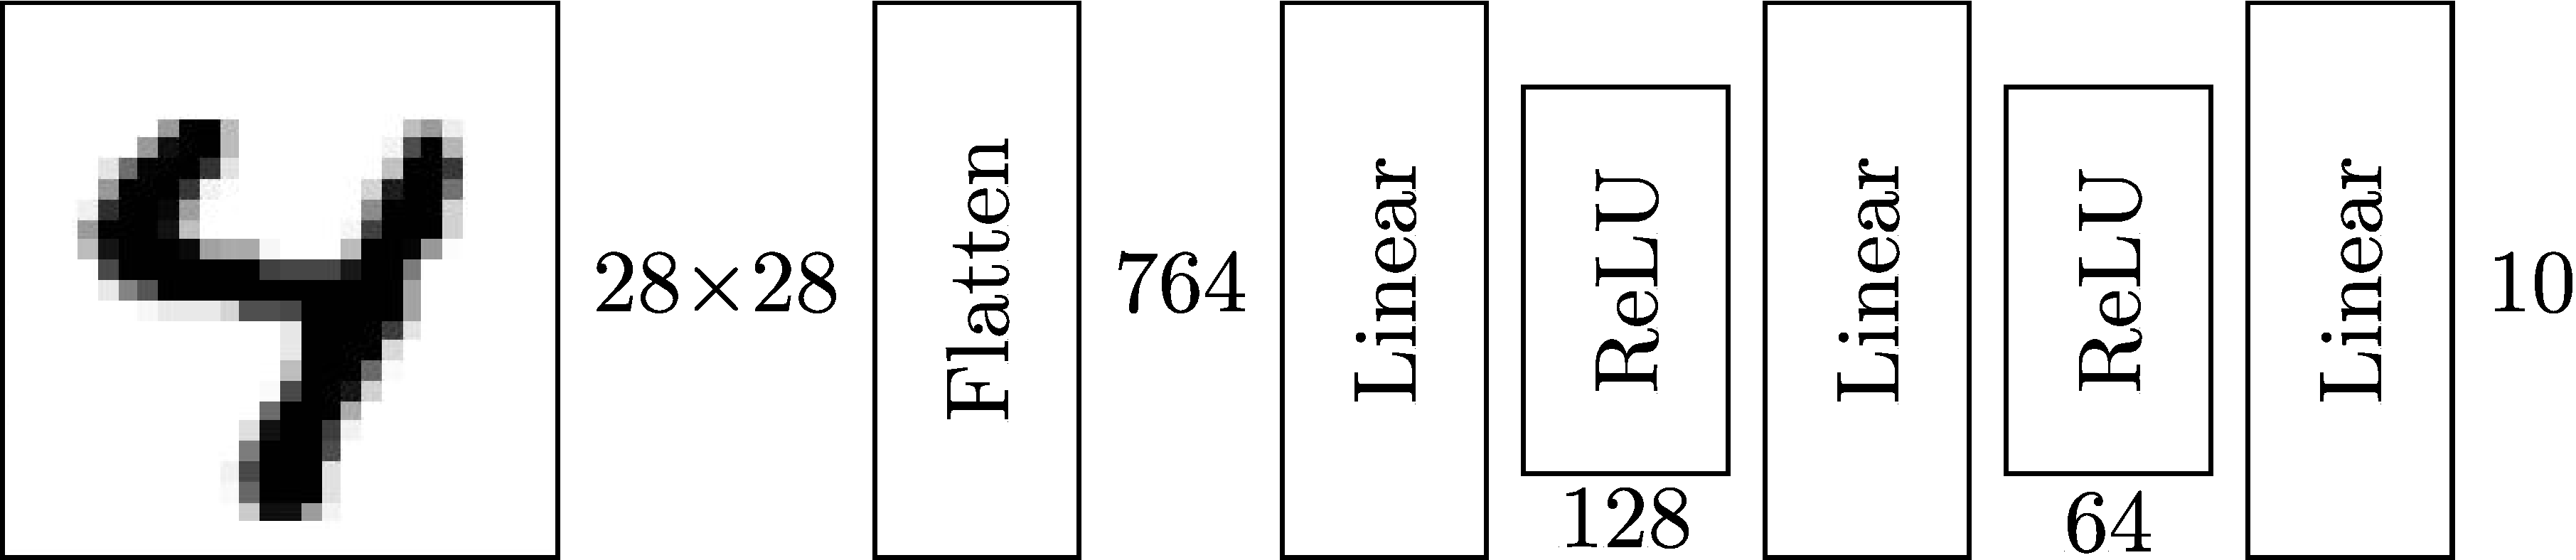
\includegraphics[width=0.7\textwidth]{model.pdf}
\end{figure}

The cross-entropy loss is used with L2 regularization.
We found that using \texttt{NLLLoss}, \texttt{Log}, and \texttt{Softmax} separately
resulted in numerical instability and NaN values during training,
so the fused \texttt{CrossEntropyLoss} operator was used directly.
\[
  \begin{aligned}
    \mathcal{L}(\theta; I, p) &= \mathcal{L}_\text{class}(\theta; I, p) + \lambda_\text{L2} \mathcal{L}_\text{L2}(\theta) \\
    \mathcal{L}_\text{class}(\theta; I, p) &= \texttt{CrossEntropy}\bigl(f_\theta(I_i), p_i\bigr) = -\sum p_i \log\Bigl( \texttt{Softmax}\bigl(f_\theta(I_i)\bigr) \Bigr)\\
    \mathcal{L}_\text{L2}(\theta) &= \sum_{W \in \theta} \norm{W}_2^2 \\
  \end{aligned}
\]

% TODO - include a abstract image of mlp or a few lines of description about the model
% How about the MLP code?

The model is trained for 10 epochs with a batch size of 100 and a learning rate of 0.1 via SGD.
We report our results on varying $\lambda_\text{L2}$ values below, taking the mean of 50 runs for each setting.

% TODO - include the result image, acc and loss
\begin{table}[h]
  \centering
  \begin{tblr}{colspec={r *{7}c}}\toprule
    $\lambda_\text{L2}$  & 0     & $10^{-7}$ & $10^{-6}$ & $10^{-5}$ & $10^{-4}$ & $10^{-3}$ & $10^{-2}$\\
    Acc. \% ($\uparrow$) & 97.23 & 97.17     & 97.26     & 97.24  & 97.21    & 96.74         & 90.81    \\
    \bottomrule
  \end{tblr}
\end{table}
We conclude that L2 regularization is not necessary in this problem.
While $\lambda_\text{L2} = 10^{-6}$ did give the best results,
the improvements were marginal and could be attributed to stochasticity.
Large $\lambda_\text{L2}$ values were significantly detrimental to training.
We attribute this to the low parameter count and the short training duration.

\printbibliography

\end{document}
